
%(BEGIN_QUESTION)
% Copyright 2011, Tony R. Kuphaldt, released under the Creative Commons Attribution License (v 1.0)
% This means you may do almost anything with this work of mine, so long as you give me proper credit

\noindent
{\bf Programming Challenge and Comparison -- Remote PLC ``stop'' button for motor control system} 

\vskip 10pt

Suppose we have an application where two PLCs are connected via a network cable.  PLC 1 directly connects to the momentary-contact ``Start'' pushbutton, ``Stop'' pushbutton, and contactor coil for a simple motor control system.  PLC 2 has its own ``Stop'' pushbutton connected, which is supposed to cause the motor at the first PLC to stop when pressed.  An HMI connected to PLC 2 reads the status of the motor (whether it is running or stopped):

$$\includegraphics[width=15.5cm]{i02492x01.eps}$$

\vskip 10pt

Work individually or in teams to write a PLC program using network communication instructions to perform the functions of remote stop and remote viewing of motor status.  {\it Note: some PLC models are unable to act as network ``master'' devices, such as the Allen-Bradley MicroLogix 1000 series A and B PLCs.}

\vskip 10pt

When your program is complete and tested, capture a screen-shot of it as it appears on your computer, and prepare to present your program solution to the class in a review session for everyone to see and critique.  The purpose of this review session is to see multiple solutions to one problem, explore different programming techniques, and gain experience interpreting PLC programs others have written.  When presenting your program (either individually or as a team), prepare to discuss the following points:

\begin{itemize}
\item{} Identify the ``tag names'' or ``nicknames'' used within your program to label I/O and other bits in memory
\item{} Follow the sequence of operation in your program, simulating the system in action
\item{} Identify any special or otherwise non-standard instructions used in your program, and explain why you decided to take that approach
\item{} Show the comments placed in your program, to help explain how and why it works
\item{} How you designed the program (i.e. what steps you took to go from a concept to a working program)
\end{itemize}

\vfil 

\vskip 20pt \vbox{\hrule \hbox{\strut \vrule{} {\bf Suggestions for Socratic discussion} \vrule} \hrule}

\begin{itemize}
\item{} Why can't communication instructions be continuously ``energized'' in PLC programs, but rather must be only occasionally activated (i.e. a series contact closing for one scan every so often)?
\item{} Does it matter which PLC is the master and which is the slave in this application?
\end{itemize}

\underbar{file i02492}
\eject
%(END_QUESTION)





%(BEGIN_ANSWER)

For Koyo CLICK PLCs, the ``Receive'' and ``Send'' instructions are fairly self-explanatory.  

\vskip 20pt

For Allen-Bradley MicroLogix PLCs, the ``Message'' (MSG) instruction is the one to use, configured for ``500CPU'' Communication Command type.  Follow these steps to ensure good operation:

\begin{itemize}
\item{} Configure the two PLCs which will be networked to each other via Ethernet with compatible IP addresses and subnets (e.g. {\tt 192.168.0.5} and {\tt 192.168.0.7}, each with a subnet mask of {\tt 255.255.255.0}).
\vskip 5pt
\item{} Either connect the two MicroLogix PLCs with a single Ethernet cable, or plug them into an Ethernet hub, allowing a laptop to still be connected to them for programming and monitoring purposes.
\vskip 5pt
\item{} Create a new ``Message'' file (e.g. {\tt MG9}) and a new ``Routing Information'' file (e.g. {\tt RI10}).  These will need to be referenced within the setup screen of the MSG instruction.
\vskip 5pt
\item{} Reference this new Message file in the MSG instruction box (e.g. MSG File = {\tt MG9:0}).
\vskip 5pt
\item{} Double-click the words ``Setup Screen'' in the MSG instruction box to access the setup screen where you may enter all the other configuration data for this instruction.
\vskip 5pt
\item{} Under the ``This Controller'' section, select Channel 1 (if you double-click on the entry field, a pull-down arrow appears, allowing you to select among options).
\vskip 5pt
\item{} Under the ``This Controller'' section, set the ``Communication Command'' to either {\tt 500CPU Read} or {\tt 500CPU Write}, depending on whether you wish to have the MSG instruction read (receive) data from another PLC, or write (send) data to another PLC.
\vskip 5pt
\item{} Under the ``This Controller'' section, set the ``Data Table Address'' to the memory location within this PLC accessed by the MSG instruction.  If you are writing information to another PLC, this is the register where the transmitted data will come from.  If you are reading information from another PLC, this is the register where the received data will be placed.
\vskip 5pt
\item{} Under the ``This Controller'' section, set the ``Size in Elements'' for the number of contiguous registers you wish to write or read.  If you only wish to read or write a single 16-bit register, leave this parameter set for 1.
\vskip 5pt
\item{} Under the ``Target Device'' section, set the ``Data Table Address'' to the memory location within the other PLC accessed by the MSG instruction.  If you are writing information to another PLC, this is the register in the other PLC where the transmitted data will be written to.  If you are reading information from another PLC, this is the register in the other PLC where the received data will be read from.
\vskip 5pt
\item{} Under the ``Target Device'' section, select {\tt Local}.
\vskip 5pt
\item{} Under the ``Target Device'' section, specify the Routing Information file you created earlier (e.g. {\tt RI10:0}).
\vskip 5pt
\item{} Select the MultiHop tab on the Setup Screen window, and there specify the IP address of the target device (i.e. the IP address of the other PLC).
\end{itemize}


%(END_ANSWER)





%(BEGIN_NOTES)

Regardless of the brand of PLC, students need to avoid connecting the input of their communication instruction straight to the ``rail'' in their programs.  Instead, the communication instruction(s) need to receive ``pulsed'' inputs (ideally lasting one scan per pulse) in order that the instruction does not collide with itself over subsequent scans.




\vfil \eject

\noindent
{\bf Summary Quiz:}

(The recommended summary quiz is to have \underbar{each student} demonstrate their PLCs running this particular program)

%INDEX% PLC, programming challenge: remote PLC stop button for motor control system

%(END_NOTES)


